\exo{\bareme1}{Calculer}

Effectuer les calculs suivants en détaillant les étapes.

\begin{multicols}{2}
    \cnt
    \begin{align*}
      &12-1+3\times 2\\
      =&12-1+6\\
      =&11+6\\
      =&17
    \end{align*}

    \columnbreak
    \cnt
    \begin{align*}
      &(7\times (2+3)-5):6\\
      =&(7\times 5-5):6\\
      =&(35-5):6\\
      =&30:6\\
      =&5
    \end{align*}
\end{multicols}

\begin{multicols}{2}
    \exo{\bareme2}{Chercher}
    
    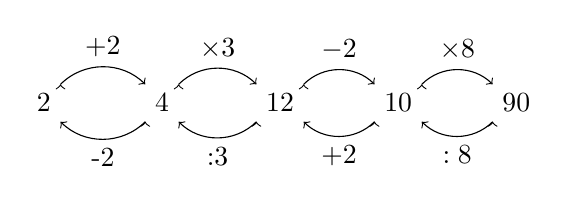
\begin{tikzpicture}[->, node distance=1.5cm]
      \node (A) {2};
      \node [right of=A] (BB) {4};
      \draw (A.north east) edge [bend left=45] node  [midway,above] {$+2$} (BB.north west) ;
      \draw (BB.south west) edge [bend left=45] node  [midway,below] {-2} (A.south east) ;


      \node [right of=BB] (B) {12};
      \draw (BB.north east) edge [bend left=45] node  [midway,above] {$\times 3$} (B.north west) ;
      \draw (B.south west) edge [bend left=45] node  [midway,below] {:3} (BB.south east) ;

      \node [right of=B] (C) {10};
      \draw (B.north east) edge [bend left=45] node  [midway,above] {$-2$} (C.north west) ;
      \draw (C.south west) edge [bend left=45] node  [midway,below] {$+2$} (B.south east) ;

      \node [right of=C] (D) {90};
      \draw (C.north east) edge [bend left=45] node  [midway,above] {$\times 8$} (D.north west) ;
      \draw (D.south west) edge [bend left=45] node  [midway,below] {$:8$} (C.south east) ;
  \end{tikzpicture}
    \columnbreak

    \exo{\bareme3}{Chercher}
  
    
    $(2+3)\times 5-1=24$
\end{multicols}

\begin{multicols}{2}
    \exo{\bareme4}{Modéliser}\\    
    Le Calcul est :$50-13+3\times 2$
    
    \columnbreak
    \exo{\bareme5}{Communiquer}
    
    Le calcul en gras a été fait avant la paranthèse.
    \begin{align*}
        &10-(1+3\times 2)\\
        =&\textbf{10-}(\textbf{1}+6)\\
        =&\textbf{9}+6\\
        =&15
    \end{align*}
\end{multicols}